%!TEX root = ../montravail.tex

\begin{titlepage}

\begin{center}

%Logo der Fachhochschule K�ln
\begin{figure}[!ht]
	\centering
		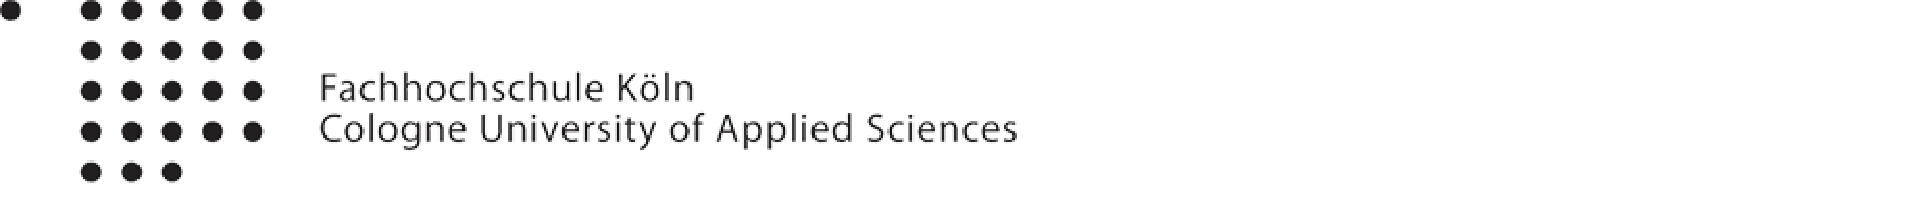
\includegraphics[natwidth=920pt, natheight=95pt, width=1.0\textwidth]{grafiken/logoheader.pdf}
\end{figure}

\vspace{0.8cm}

%Deutscher Titel
\begin{rmfamily}
%\textbf{\huge Transmover}\\
%\vspace{0.2cm}
\textbf{\huge DSL specification implementation TTCN3 \\ Domain Specific Language}\\
\normalsize
\end{rmfamily}
%
%\vspace{0.8cm}
%
%%Englischer Titel
%\begin{rmfamily}
%\textbf{Transmover}\\
%\large Development of a programmatic support exoskeleton robot \\and prototype implementation as a model\\
%\normalsize
%\end{rmfamily}

\vspace{1.2cm}

%Diplomarbeit 
%\begin{LARGE}
%\begin{scshape}
%\textbf{Diplomarbeit}\\[0.8em]
%\end{scshape}
%\end{LARGE}


\begin{LARGE}
\textbf{Master Thesis}\\
\end{LARGE}


\vspace{0.4cm}

%ausgearbeitet von...
\begin{large}
%Transmover\\
Author\\ 
\vspace{0.2cm}
\begin{LARGE}
\textbf{El Mehdi Bennani}\\
\end{LARGE}
\end{large}

%\vspace{0.6cm}
%
%%zur Erlangung des akademischen Grades...
%\begin{large}
%zur Erlangung des akademischen Grades\\
%\vspace{0.2cm}
%\textsc{Diplom Technischer Informatiker}\\
%\end{large}

\vspace{1.2cm}

%vorgelegt an der...
\begin{small}
vorgelegt an der\\ 
\vspace{0.4cm}
%\begin{scshape}
Fachhochschule K�ln\\
University of Applied Sciences Cologne\\
07 Fakult�t f�r Informations-, Medien- und\\
Elektrotechnik\\
%\end{scshape}
\end{small}

\vspace{1.2cm}

%im Studiengang...
\begin{small}
im Studiengang\\ 
\vspace{0.4cm}
%\textsc{
Technische Informatik \\
Matrikelnummer: 11033253 
\end{small}


\vspace{2.0cm}

%Autor der Masterarbeit und die Pr�fer
\begin{tabular}{rl}
        Erster Pr�fer:  &  Prof. Dr. Hans W. Nissen\\
       							    &  \small Fachhochschule K�ln \\[1.0em]
       Zweiter Pr�fer:  &  Professor Dr. Holger G�nther \\
       							    &  \small Fachhochschule K�ln \\
\end{tabular}

\vspace{0.6cm}

%Ort, Monat der Abgabe
\begin{large}
{\large \today}\\[4cm] % Date
%Koeln, September 2015
\end{large}

\end{center}

\newpage
\thispagestyle{empty}

%Kontaktm�glichkeiten des Autors und der Pr�fer
\begin{center}
\begin{tabular}{rl}
							&  \\[36.0em]
							
\large \textbf{Adressen:}	&  \quad El Mehdi Bennani\\
							&  \quad Mustermannstrasse 11\\
							&	 \quad 12345 Musterhausen\\
							&  \quad Muster@Muster.com\\[2.0em]
							
							&  \quad Professor Dr. Hartmut B�rwolff\\
							&  \quad Fachhochschule K�ln\\
							&  \quad Institut f�r Elektronik \\
							&  \quad und Informationsengineering\\
							&	 \quad Steinm�llerallee 1\\
							&	 \quad 51643 Gummersbach\\
							&  \quad Baerwolff@gm.fh-koeln.de\\[2.0em]
							
							&  \quad Professor Dr. Holger G�nther\\
							&  \quad Fachhochschule K�ln\\
							&  \quad Institut f�r Informatik\\
							&	 \quad Steinm�llerallee 1\\
							&  \quad 51643 Gummersbach\\
							&  \quad Guenther@gm.fh-koeln.de\\
\end{tabular}
\end{center}

\end{titlepage}
